\chapter{General Relativity and Cosmology}
\section{Motivation}
With Einstein's formulation of special relativity came a beautiful expansion of physics into the high-energy and large-scale regime. A postulate of special relativity was that light is a universal speed limit, and with this postulate, a plethora of established physical theories became problematic. Fortunately, for theories such as electromagnetism, no incompatibilities were introduced. However, for gravity, this was not the case. The gravitational field had no wave equation to establish a speed of propagation, meaning changes to the gravitational field are felt instantaneously everywhere. Attempts to reconcile this, such as using a retarded propagator or promoting the Newtonian potential to a scalar field theory, proved incapable of correcting for special relativistic effects. Nevertheless, Newtonian gravity has stood the test of time to be accurate in the non-relativistic limit. Thus, any theory of gravity should reduce to the Newtonian theory for speeds much lower than the speed of light.

The famous thought experiment of an Einstein elevator demonstrates a striking inconsistency within Newtonian gravity. Consider an observer freely falling in a spherical gravitational field pointing toward the center. With nothing in view, this person would not be able to determine they were in a gravitational field rather than just linearly accelerating. Suppose this observer has point particles nearby, one to each side, one above, and one below (figure~\ref{fig:tidal_forces}). The observer will see the particles below and above them move farther away because the gravitational force scales as $1/r^2$. They will see the particles to the side of them moving towards them due to the spherical symmetry of the gravitational field. These fictitious forces are referred to as \textit{tidal forces}, as they also give rise to the tides twice per day on earth. This interesting thought experiment shows how freely falling reference frames are not inertial frames, the first inconsistency recognized by Einstein. 
\begin{figure}
    \centering
    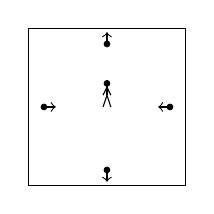
\begin{tikzpicture}
        \draw (-1,-1) -- (-1,1) -- (1,1) -- (1,-1) -- (-1,-1);
        \draw[fill=black] (0,0.3) circle (1pt);
        \draw (0,0.3) -- (0,0.15);
        \draw (0,0.15) -- (0.05,0);
        \draw (0,0.15) -- (-0.05,0);
        \draw (0,0.25) -- (0.05,0.15);
        \draw (0,0.25) -- (-0.05,0.15);
        \draw[fill=black] (-0.8,0) circle (1pt);
        \draw[fill=black] (0.8,0) circle (1pt);
        \draw[fill=black] (0,0.8) circle (1pt);
        \draw[fill=black] (0,-0.8) circle (1pt);
        \draw[->] (0,-0.8) -- (0,-0.95);
        \draw[->] (0,0.8) -- (0,0.95);
        \draw[->] (-0.8,0) -- (-0.65,0);
        \draw[->] (0.8,0) -- (0.65,0);
    \end{tikzpicture}
    \caption{Observer in free-fall, with particles experiencing tidal forces within the observer's reference frame.}
    \label{fig:tidal_forces}
\end{figure}

In the early 1900s, Einstein published his first paper on special relativity. In special relativity, physical space is enhanced to a four-dimensional space, typically denoted $\mathbb{M}^4$ or $\mathbb{R}^{3,1}$. Setting the speed of light $c=1$ (which is done in the rest of this thesis), the metric is given by
\begin{equation}
    g = \mathrm{diag}(-1,1,1,1)\,.
\end{equation}
This space is typically called \textit{Minkowski space} (thus the notation $\mathbb{M}^4$). Distances under this metric are called the \textit{proper time} interval, denoted $\tau$.
\begin{equation}\label{eq:proper-time}
    -d\tau^2 = -dt^2 + dx^2 + dy^2 + dz^2
\end{equation}
Proper time represents the amount of time that passes for an observer travelling on a path with 0 spatial displacement. Naturally, this quantity should be invariant, even for an observer in a different reference frame. For such an observer, the time that elapses will be different from $\tau$, and will be accounted for in the spatial displacement as seen by equation~\ref{eq:proper-time}. The set of transformations that leave $\tau$ invariant are the \textit{Lorentz transformations}.
\begin{figure}
    \centering
    \begin{tikzpicture}
        \draw (0,-2) -- (0,-0.5);
        \draw[dashed] (0,-0.5) -- (0,1.7);
        \draw (0,1.7) -- (0,2);
        \draw (-2,0) -- (2,0);
        \draw (0,2)  node[anchor=south] {$t$};
        \draw (2,0)  node[anchor=west] {$x$};
        \draw plot [smooth] coordinates {(-0.8,-1.5) (-0.3,-0.5) (0,0) (0.4,0.7) (-0.3,1.7) (-0.2,2.0)};
        \draw[fill=black] (-0.3,-0.5) circle (1pt);
        \draw[fill=black] (-0.3,1.7) circle (1pt);
        \draw[very thick] plot [smooth] coordinates {(-0.3,-0.5) (0,0) (0.4,0.7) (-0.3,1.7)};
        \draw (0.3,0.7) node [anchor=west] {$\Delta \tau$};
        \draw[fill=black] (0,-0.5) circle (1pt);
        \draw[fill=black] (0,1.7) circle (1pt);
        \draw (0,0.6) node [anchor=east] {$\Delta t$};
    \end{tikzpicture}
    \caption{Definition of proper time (bold line) vs. coordinate time (dashed line).}
\end{figure}

Suppose there are two observers, one is in an inertial frame with coordinates $x$ and the other is in a non-inertial frame with coordinates $x'$. These coordinates are related $x = x(x')$. In the inertial frame, the equations of motion are given by 
\begin{equation}
    \frac{d^2x^\mu}{d\tau^2} = 0\,.
\end{equation} 
One can look at how this changes for the observer in a non-inertial frame:
\begin{equation}\label{eq:sr-curves}
    \frac{d^2x'^\lambda}{d\tau^2}+\underbrace{\frac{\partial x'^\lambda}{\partial x^\rho}\frac{\partial^2 x^\rho}{\partial x'^\mu \partial x'^\nu}}_{\equiv \Gamma_{\mu\nu}^\lambda} \frac{d x'^\mu}{d \tau} \frac{d x'^\nu}{d \tau} = 0\,.
\end{equation}
Equation~\ref{eq:sr-curves} looks suspiciously like the geodesic equation from differential geometry. The exception is that the `Chirstoffel symbols', as defined here, are not the most general form of the Christoffel symbols. This gives motivation for how to search for a compatible theory of gravity by providing a clear link between gravity and geometry. 
\section{Einstein's Field Equation}
Christoffel symbols take a very general form, where they signify the failure of derivatives to commute, which results from curvature of the space itself. Special relativity promotes the classical $\mathbb{R}^3$ space to $\mathbb{M}^4$. However, the metric must allow for curved space, not simply Minkowski space. Instead of $\mathbb{M}^4$, let space be an arbitrary semi-Riemannian 4-manifold $M$ with a metric with one negative eigenvalue.\footnote{In very loose terms, a manifold is a locally Euclidean space, which is a sufficient definition for this application.}

Naturally, computing derivatives on curved surfaces is non-trivial, as there is no way to compare tangent vectors at two different points of a manifold. One can, however, use the fact that derivatives give tangent vectors and look at a single point $p\in M$ to construct the tangent space at $p$, denoted $T_pM$. The generalization of the derivative is called a \textit{connection}~\cite{baez_john_gauge_1994}, which tells one how to connect the tangent spaces at different points infinitesimally (figure~\ref{fig:parallel_transport}). Although beyond the scope of this thesis, it is worth noting that, due to the holonomy of curved surfaces, this will generally depend on the path taken.
\begin{figure}
    \centering
    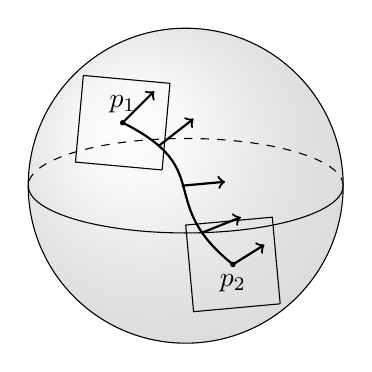
\begin{tikzpicture}
        \shade[ball color = gray!40, opacity = 0.2] (0,0) circle (2cm);
        \draw (0,0) circle (2cm);
        \draw (-2,0) arc (180:360:2 and 0.6);
        \draw[dashed] (2,0) arc (0:180:2 and 0.6);
        \fill[fill=black] (-0.8,0.8) circle (1pt);
        \draw (-0.8,0.8) node[anchor=south] {$p_1$};
        \fill[fill=black] (0.6,-1.0) circle (1pt);
        \draw (0.6,-1.0) node[anchor=north] {$p_2$};
        \draw (-0.8+0.5,0.8-0.6) -- (-0.8-0.6,0.8-0.5) -- (-0.8-0.5,0.8+0.6) -- (-0.8+0.6,0.8+0.5) -- (-0.8+0.5,0.8-0.6); %bottom right -- bottom left -- top left -- top right -- bottom right
        \draw (0.6+0.6,-1-0.5) -- (0.6-0.5,-1-0.6) -- (0.6-0.6,-1+0.5) -- (0.6+0.5,-1+0.6) -- (0.6+0.6,-1-0.5);
        \draw[thick] (-0.8,0.8) .. controls (0.4,0.2) and (-0.4,-0.2) .. (0.6,-1);
        \draw[->,thick] (-0.8,0.8) -- (-0.4,1.2);
        \draw[->,thick] (-0.35,0.5) -- (0.1,0.85);
        \draw[->,thick] (-0.05,0) -- (0.5,0.05);
        \draw[->,thick] (0.2,-0.6) -- (0.7,-0.4);
        \draw[->,thick] (0.6,-1) -- (1,-0.75);
    \end{tikzpicture}
    \caption{Example of parallel transport along a connection on a sphere. }
    \label{fig:parallel_transport}
\end{figure}
In general relativity, a special connection is used called the \textit{Levi-Civita connection}, denoted $\nabla$, which is torsionless and metric preserving. That is, for all vector fields $u,v,w$ on $M$
\begin{equation}
    \begin{array}{lr}
        u g(v,w) = g(\nabla_u v, w)+g(v,\nabla_u w) \,, & \text{(metric preserving)} \,, \\
        u,v = \nabla_u v - \nabla_v u \,, & \text{(torsion free)}\,. \\
    \end{array}
\end{equation}

The only remaining geometric property for the Levi-Civita connection is curvature, which can be neatly described using the Christoffel symbols defined by
\begin{equation}
    \nabla_\mu\partial_\nu = \Gamma^{\rho}_{\mu\nu}\partial_\rho\,.
\end{equation}
In this case, the partials here are referring to the basis of vector fields on $M$. Additionally, this curvature has a special name as well, the \textit{Riemann curvature}, a type (3,1) tensor defined by
\begin{equation}
    R(u,v)w = (\nabla_u\nabla_v-\nabla_v\nabla_u - \nabla_{[u,v]})w\,,
\end{equation}
or in coordinate form by
\begin{equation}
    R_{\mu\nu\rho}^\sigma  = \nabla_\mu \Gamma^\sigma_{\nu\rho} - \nabla_\nu\Gamma^{\sigma}_{\mu\rho}\,.
\end{equation}
To emphasize the elegance of Einstein's equation, it is convenient to write the Riemann curvature as a matrix valued differential 2-form $F$ and the Christoffel symbols as a matrix valued differential 1-form\footnote{Differential forms are antisymmetric contravariant tensors.} $\mathcal{G}$~\cite{baez_john_gauge_1994}. With this notion, it is easy to see the Bianchi identity for $F$ with respect to the Levi-Civita connection is
\begin{equation}
    d_{\nabla}F = \nabla_{[\tau}R^\sigma_{\mu\nu]\rho} = 0\,,
\end{equation}
where the brackets denote antisymmetric permutations of the indices. Working through the algebra gives
\begin{equation}
    \nabla^\mu G_{\mu\nu} = 0\,,\quad G_{\mu\nu} = R_{\mu\nu}-\frac{1}{2}g_{\mu\nu}R\,,
\end{equation}
where $R$ and $R_{\mu\nu}$ are the Ricci scalar and Ricci tensor, found by contracting indices in the Riemann tensor. This looks familiar to the conservation of energy equation,
\begin{equation}
    \nabla^\mu T_{\mu\nu}=0\,.
\end{equation}
Additionally, the metric itself is divergenceless. Putting these all together gives us Einstein's Field Equation
\begin{equation}
    G_{\mu\nu} + \Lambda g_{\mu\nu} = 8\pi\kappa T_{\mu\nu}\,.
\end{equation}

\section{Cosmology}
Einstein's equation includes the constant $\Lambda$, which is called the \textit{cosmological constant}. A great question in gravitational physics and cosmology is `what value does $\Lambda$ take, and what is its source'. The theory of $\Lambda$CDM, the standard model of cosmology, will be discussed, where dark matter is `cold' (so it clumps to form halos) and dark energy acts as the cosmological constant~\cite{scott_dodelson_modern_2021}.

When discussing $\Lambda$CDM (or cosmology in general), there are two main assumptions that are made on a global scale:
\begin{itemize}
    \item The universe is \textit{homogeneous}. That is, there is no preferred location in the universe.
    \item The universe is \textit{isotropic}. That is, there is no preferred direction of the universe.
\end{itemize}
Both of these assumptions should sound strange; Our universe clearly does not follow them. If one looks into the night sky, one can see regions of densely packed stars and galaxies and other regions with no stars or galaxies, violating the assumption of homogeneity (figure~\ref{fig:galaxy_map}). On the other hand, if one observes the temperature of the cosmic microwave background (CMB), one finds there is an angle dependence of the observed temperature (figure~\ref{fig:cmb_tt_map}), violating the assumption of isotropy. To reconcile this, the metric will be modified by perturbations. In this thesis, only scalar perturbations are considered.
\begin{figure}[ht]
    \centering
    \includegraphics[width=0.75\textwidth]{plots/weic2305a.jpg}
    \caption{An image of galaxies from the James Webb Space Telescope, showing regions of high matter density and regions of low matter density~\cite{webb_clusters}.}
    \label{fig:galaxy_map}
\end{figure}
\begin{figure}[ht]
    \centering
    \includegraphics[width=0.75\textwidth]{plots/Planck_CMB.jpg}
    \caption{CMB temperature map, emphasizing the scale of anisotropies~\cite{planck_CMB}.}
    \label{fig:cmb_tt_map}
\end{figure}

With Edwin Hubble's discovery of the expanding universe, any metric assigned to the universe must include homogeneous spatial expansion. Together with the above assumptions, one arrives at the Friedmann-Lema\^{i}tre-Robertson-Walker (FLRW) metric in the Newtonian gauge,
\begin{equation}
    g = -dt^2 + a(t)^2 ds^2\,,
\end{equation}
where $s$ represents spatial coordinates. Working in the Newtonian gauge is chosen to best illuminate the physics discussed throughout this thesis. To perturb this metric around a homogeneous universe, it requires two fields. The first, denoted $\Psi$, is the Newtonian gravitational potential. Because Newtonian gravity works in the non-relativistic limit, it enters the time component of the metric. The second field, denoted $\Phi$, represents spatial curvature perturbations. The perturbed metric is given by
\begin{equation}
    g = -(1+2\Psi)dt^2 + a^2(1-2\Phi)ds^2\,.
\end{equation}
By computing the Christoffel symbols, one finds
\begin{equation}
    \begin{split}
        \Gamma^i_{00} =& \frac{1}{a^2}\partial_i\Psi \\
        \Gamma^i_{0j} =& \delta_{ij}(H+\dot\Phi) \\
        \Gamma^i_{jk} =& (\delta_{ij} \partial_k + \delta_{ik}\partial_j - \delta_{jk}\partial_i)\Phi\,.
    \end{split}
\end{equation}
Given Einstein's field equations and the perturbed FLRW metric, one can find the Friedman equations. The first comes from the $00$ component of Einstein's field equations:
\begin{equation}
    H^2(t) = \frac{8\pi G}{3}\left(\rho + \frac{\Lambda}{8\pi G}\right) - \frac{k}{a^2}\,.
\end{equation}
One can convert the curvature $k$ and the cosmological constant $\Lambda$ into densities as well, denoted $\rho_k$ and $\rho_\Lambda$ respectively. If those terms are absorbed into the total density $\rho$, one finds
\begin{equation}
    H^2(t) = \frac{8\pi G}{3}\rho\,,
\end{equation}
and the critical density today is defined by the density associated with $H_0$,
\begin{equation}
    H_0^2 \equiv \frac{8\pi G}{3}\rho_{\mathrm{crit}}\,.
\end{equation}
The desirable property of this formulation is that the value of the density today can tell us about the geometry of the universe. If $\rho>\rho_{\mathrm{crit}}$ the curvature is positive (de Sitter geometry). If $\rho<\rho_{\mathrm{crit}}$ the curvature is negative (anti-de Sitter geometry). If $\rho=\rho_{\mathrm{crit}}$, the universe is flat. If one defines the relative densities today by
\begin{equation}
    \Omega_{i,0} = \frac{\rho_{i,0}}{\rho_\mathrm{crit}}\,,
\end{equation}
the relation becomes
\begin{equation}
    \Omega + \Omega_k = 1 \,,
\end{equation}
meaning if the non-curvature relative densities are less than 1, then the universe is curved with sign equal to the sign of $\Omega_k$. 
% This relates to the way we determine distances in the universe. The corresponding distance is called the \textit{angular distance}, relating the angle subtended by two rays to the distance between them. This depends on the geometry of the universe and depends on the physical distance $D$ and the radius of curvature $R$.
% \begin{equation}
%     D_A = \left\{ \begin{array}{cc}
%         R & K=0 \\
%         R\sin(D/R) & K>0 \\
%         R\sinh(D/R) & K<0
%     \end{array}
%     \right.\,.
% \end{equation}
The second Friedman equation comes from the trace of Einstein's equation,
\begin{equation}
    \frac{\ddot a}{a} = -\frac{4\pi G}{3}(\rho + 3P)\,.
\end{equation}
In cosmology, there are other distances which can be more useful than the distance given by the FLRW metric. In the FLRW metric, the distance between two points grows in time. 
This can be avoided by defining the \textit{comoving distance}, in which distances remain fixed through time. 
If one looks at a coordinate function $x^\mu$ at $t=t_0$, at a later time the coordinate function can be written as $x^\mu \rightarrow a(t) x^\mu$, thus by dividing by the scale factor $a(t)$  one can define the comoving coordinates as
\begin{equation}
    \chi = \int\limits^{t}_{t_0} \frac{1}{a(t')} dt'
\end{equation}
with the standard Minkowski metric multiplied by the scale factor $a$. This can be taken a step further by determining the distance light has travelled since $t=0$, called the \textit{comoving horizon}, by
\begin{equation}
    \eta = \int\limits^t_0 \frac{1}{a(t')}dt'\,.
\end{equation}

This chapter provides a brief overview of the relevant pieces of cosmology that will be used throughout the rest of this thesis. The next two chapters will use these pieces to see how one can measure cosmological parameters from cosmological surveys. The fourth chapter will be a study on a parameter splitting technique, which provides a model independent consistency check in $\Lambda$CDM. The fifth chapter provides a study of applying neural networks to cosmological analysis, and a scientific application to the evaluation of cosmological tensions.